{
\large
\textbf
{
Transportarbeid (inkl trafikksikkerhet, klimagassutslipp og vegslitasje mv)
}
}

\begin{formal}
Mål: 15-20 \% redusert antall transport-turer som følge av 74 tonn sammenlignet med 60 tonn vogntog
\end{formal}

For å se på reduksjonen i antallet tranport-turer, så er det her tatt utgangspunkt i den prosentvise
reduksjonen i påkrevde transport-turer mellom referanseekvipasjen (60T) og samtlige andre ekvipasjer.
Antallet påkrevde transport-turer kan finnes som forholdet mellom antall enheter som skal tranporteres og
kapasiteten per tur. 
Figur \ref{fig:timer_per_trip} viser estimerte fordelinger av last-kapasiteten til hver ekvipasje,
utarbeidet ved å trekke kjøretøyenes basevekt fra kjøretøyenes totalvekt.

\begin{figure}[H]
\centering
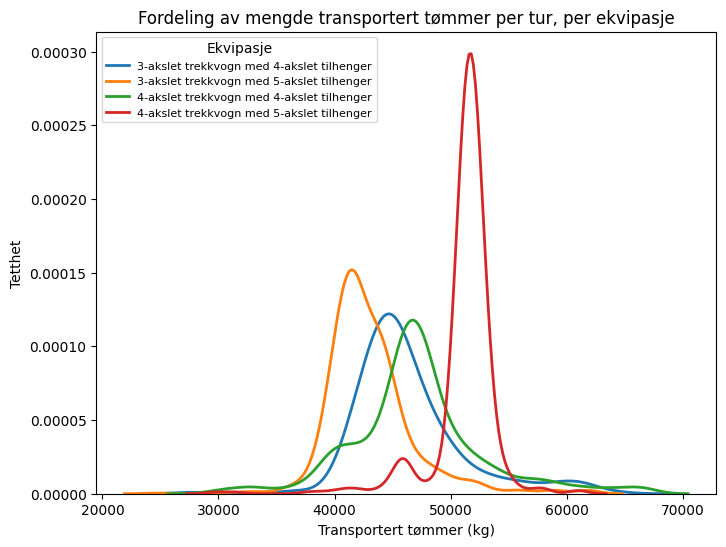
\includegraphics[width=0.5\textwidth]{images/timer_per_trip.png}
\caption{Estimerte fordelinger av lastkapasitet}
\label{fig:timer_per_trip}
\end{figure}

\phantom{}\\
Dersom man tar utgangspunkt i
snittverdiene til disse fordelingene og regner på prosentvis reduksjon i antallet transport-turer, altså:

\[
100 \cdot \left(\frac{ \frac{enheter}{referansekapasitet} - \frac{enheter}{kapasitet} }{\frac{enheter}{referansekapasitet}}\right)
\]
\\
\[
= 100 \cdot \left( 1 - \left(\frac{referansekapasitet}{kapasitet}\right) \right)
\]

\phantom{}\\
Så ender man opp med følgende resultater:

\begin{table}[H]
    \resizebox{\textwidth}{!}{%
    \begin{tabular}{lrrr}
        \toprule
        ekvipasje & Tømmer (kg) gjennomsnitt & Gj.snitt forskjell (\%) & Turreduksjon gj.snitt (\%) \\
        \midrule
        3-akslet trekkvogn med 4-akslet tilhenger & 46369.980000 & 0.000000 & 0.000000 \\
        3-akslet trekkvogn med 5-akslet tilhenger & 43051.230000 & -7.160000 & -7.710000 \\
        4-akslet trekkvogn med 4-akslet tilhenger & 47083.490000 & 1.540000 & 1.520000 \\
        4-akslet trekkvogn med 5-akslet tilhenger & 51203.690000 & 10.420000 & 9.440000 \\
        \bottomrule
        \end{tabular}
    }
    \caption{Prosentvise reduksjoner i antallet transport-turer sammenliknet med referanseekvipasjen på 60 tonn}
    \label{tab:transportanalyse}
\end{table}

\phantom{}\\
Resultatene viser at 74T ekvipasjen reduserer antallet påkrevde transport-turer med rundt 9.4\%, 68T med 1.62\%, og at 65T \textit{øker} antallet påkrevde turer med drøye 7.7\%.
Det siste funnet virker noe tvilsomt, og skyldes trolig en kombinasjon av at 60T ekvipasjene laster opp slik at totalvekt blir tilnærmet lik som for 65T (illustrert i Figur \ref{fig:boxplot_totalweights})
og skjevheter i datagrunnlaget.

\begin{formal}
Reduserte CO2 utslipp med 10 \%
\end{formal}

\phantom{}\\
Tar man utgangspunkt i den estimerte mengden transportert tømmer for hver loggede kjøretøy, for deretter å sette opp
mengden Co2 sluppet ut mot tonn-kilometer av tømmer, ender man med den følgende tilnærmede fordelingen:

\begin{figure}[H]
    \centering
    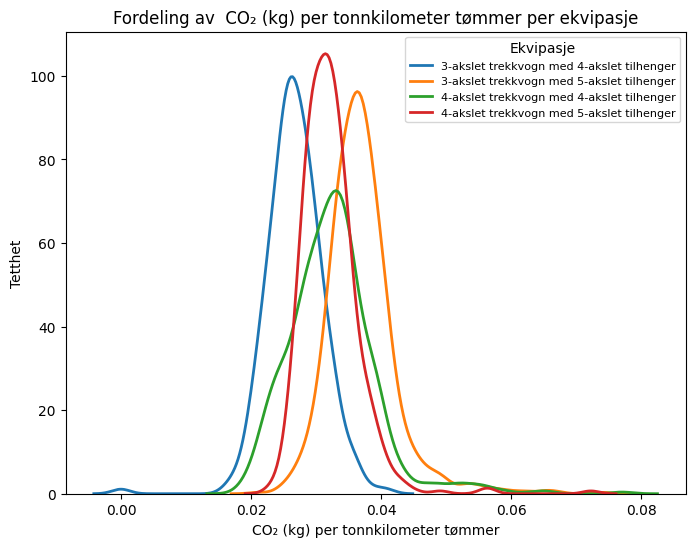
\includegraphics[width=0.75\textwidth]{images/co2_per_tonnagedistance.png}
    \caption{Analyse av transportarbeid for ulike ekvipasjer}
    \label{fig:co2_per_tonnagedistance}
\end{figure}

Snittet av disse fordelingene satt opp mot referansen (60T) gir følgende resultater:

\begin{table}[H]
    \resizebox{\textwidth}{!}{%
    \begin{tabular}{lrr}
        \toprule
        ekvipasje & Co2 (kg) per tonnkilometer tømmer snitt & Endring Co2 gj.snitt (\%) \\
        \midrule
        3-akslet trekkvogn med 4-akslet tilhenger & 0.026730 & 0.000000 \\
        3-akslet trekkvogn med 5-akslet tilhenger & 0.036990 & 38.369050 \\
        4-akslet trekkvogn med 4-akslet tilhenger & 0.032500 & 21.564160 \\
        4-akslet trekkvogn med 5-akslet tilhenger & 0.032170 & 20.360140 \\
        \bottomrule
        \end{tabular}
    }
    \caption{Analyse av lastevolum og reduksjon i antall transportturer}
    \label{tab:co2_tonkm}
\end{table}

\phantom{}\\
Dette viser at de tyngre ekvipasjene slipper ut mer Co2 per transportert mengde tømmer. Dette skyldes trolig
utbredt overvektskjøring blant 60T ekvipasjen (Som vist i Figur \ref{fig:boxplot_totalweights}), som medfører
at en større andel av totalvekten går til tømmer og ikke selve kjøretøyet.

\begin{formal}
Nedbrytning av veg og slitasje på bruer skal ikke øke utover dagens situasjon gittsamme transportarbeid
\end{formal}
Dette har foreløpig ikke blitt undersøkt.

\begin{formal}
Trafikksikkerhet: Ingen skader eller ulykker med materiell eller personskader somfølge av prøveordningen
\end{formal}
Dette har foreløpig ikke blitt undersøkt.

{
\large
\textbf
{
Lønnsomhet for næringen
}
}

\begin{formal}
Mål: 10 \% reduserte transportkostnader og drivstofforbruk for tømmernæringen somfølge av 74 tonn sammenlignet med transportkostnader og drivstofforbruk med 60tonn vogntog.
\end{formal}
Dette har foreløpig ikke blitt undersøkt.
